\documentclass{article}

\usepackage[utf8x]{inputenc}
\usepackage[spanish]{babel}
\usepackage[margin=3cm]{geometry}
\usepackage{amsmath}
\usepackage{amssymb}

\usepackage{graphicx}

\linespread{1.2}

\title{Computación Concurrente \\ \Large{Tarea 3}}
\author{
  Diego Goméz Montesinos
  \and
  José Emiliano Cabrera Blancas
  }
\date{25 febrero 2014}
\begin{document}
\maketitle
\begin{enumerate}
\item{
    \textsl{
    Recuerden el modelo visto en clase con el que resolvimos la tarea
    $\epsilon$-aggremment para dos procesos. Alice y Bob proponen un valor y
    quieren quedar de acuerdo en un valor que no diste más de $\epsilon$ de lo
    que el otro decidió. Después vimos que necesitaban comunicarse y que para 
    $\epsilon$ más pequeñas se necesitaban mñas y más rondas de comunicación.
    Recuerden que usamos el modelo de memoria compartida de lectura/escrita por
    capas \textit{full information} (por cada escritura leiamos un nuevo
    arreglo y escribimos todo lo que sabemos cada vez).\\
    Ahora proponemos otros dos modelos de comunicación: el modelo chismoso y el
    modelo discusión civil. El modelo chismoso dice que si Alice y Bob alguno de
    los 2 no escucho al otro entonces tienen otra ronda de comunicación. De lo 
    contrario. De lo contrario si los dos se escuchan entonces ahi termina la 
    comunicación. Podriamos verlo como que se lanzan insultos e indirectas pero
    no de frente.\\
    El modelo discusión civil dice que mientras Alice y Bob esten escuchando 
    mutuamente la conversación sigue. En el momento que uno ya no escucha al otro
    ahi se termina.
    Sea \textit{M} $≥$ 0 el número de rondas máximo que se pueden comunicar Alice
    y Bob:}
      
    %%\begin{center}
      %%Figura 1:\\
      %%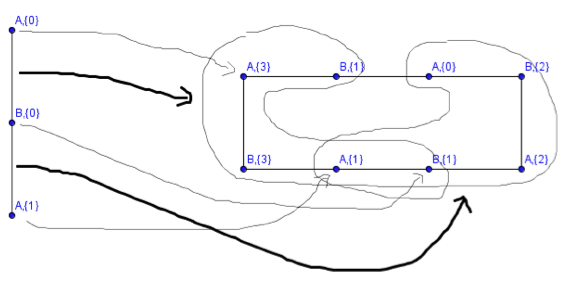
\includegraphics[scale=0.65]{Figura1.png}
    %%\end{center}

    \begin{enumerate}
      \item{\textsl{Para los 2 modelos dados describe el complejo del protocólo para M. 
        Tienes que dar la tripleta $(I,P_m,\Xi_m)$}}

      \item{\textsl{Para los 2 modelos describe cuál es la tarea $\epsilon$-agreement
        óptima para cada \textit{M} $≥$ 0. Nos referimos a óptimo como que cada
        vista del protocolo va a un valor de decisión único. En otras palabras
      encontrar la $\epsilon$ en función de M.}}
    \end{enumerate}
  }

\item{
    \textsl{
    Con el modelo visto en clase define la función de decisión de equidad de género
    $\delta$, que no distingue entre Alice y Bob. Es decir Alice y Bob pueden tener
    ya sea el valor 0 o 1 de entrada. También da la $\delta$ óptima para este caso.
    Aqui debes de tener cuidado de como etiquetas los vértices para que siempre
    se cumpla la $\epsilon$.}\\
  
    Primero vamos a cambiar el complejo de entrada de tal forma que sea más fácil 
    comprender el problema y con ello dar una $\epsilon$-agreement para M rondas.\\
    
     \begin{figure}
       \centering
       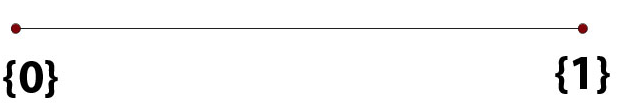
\includegraphics[scale=0.25]{2_input.png}
       \caption{Complejo de entrada para $\epsilon$-agreement con equidad de género.}
     \end{figure}

     La explicación del complejo de entrada es(\textit{figura 1}):
     
     \begin{itemize}
       \item{El vertice con etiqueta {0} representa el mundo donde al menos un proceso
           tiene como entrada 0.}
       \item{El vertice con etiqueta {1} representa el mundo donde al menos un proceso
           tiene como entrda 1.}
       \item{La arista entre los dos únicos vertices representa el mundo donde algun 
           proceso tiene como entrada 0 y otro tiene entrada 1.}
     \end{itemize}
  }

  ¿Como evoluciona este complejo en la primera ronda?, la \textit{figura 2} es la
  gráfica de protocolo de la ronda 1.

  \begin{figure}
    \centering
    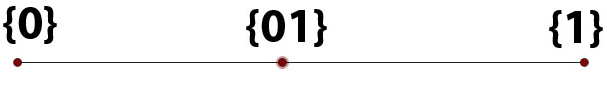
\includegraphics[scale=0.25]{2_protocol2.png}
    \caption{Gráfica de protocolo de la primera ronda  para $\epsilon$-agreement con equidad de género.}
  \end{figure}
  
  En esa gráfica tenemos tres vértices que representan lo siguiente:
  
  \begin{itemize}
    
    \item{La etiqueta {0} representa el mundo donde el o los procesos  escucharon 0 
         o no escucharon nada y como entrada tuvieron 0.}
      
    \item{La etiquieta {01} representa el mundo donde el o los procesos  escucharon 0 o 1
        y esos procesos tiene como entrada el numero contrario al que escucharon.}
      
    \item{La etiquieta {1} representa el mundo donde el o los procesos escucharon 1
      o no escucharon nada y como entrada tuvieron 1.}

    \item{Las aristas entre cada vértices representa que existe un mundo donde hay 
      vértices de un tipo y vértices del otro.}
    
  \end{itemize}

  Analizemos cuál es la $\epsilon$-agreement para la primera ronda.\\
  Como nuestra gráfica de protocolo tiene 3 vértices, entonces la $\delta(x)$
  es la siguiente:\\
  
  \begin{itemize}
    
  \item{Si x sabe que alguien dijo 0 y alguien dijo 1, entonces decide $1/2$.}
    
  \item{Si x dijo 0 y escucho 0 o no escucho nada, entonces decide $0$.}
    
  \item{Si x dijo 1 y escucho 1 o no escucho nada, entonces decide $1$.}
    
  \end{itemize}
  
  Como podemos darnos cuenta, la $\delta$-óptima es $1/2$ y no puede ser menor
  por que querría decir que existe un mapeo de un camino de 3 vértices a otro
  camino de más de 3 vértices.\\

  Ahora que ya sabemos como fue la $\Xi$ para la primera ronda, es fácil ver
  que en cada ronda las aristas se dividen en otras dos aristas, y analogmanete
  decimos que la $\delta$-óptima es $1/2^k$ pues que si existiera una $\delta$
  mejor, querria decir que existe un mapeo de un camino de $2^k$ vértices a otro
  camino de más de $2^k$ vértices.\\

  Como corolario de esto último podemos decir que el algoritmo para optener
  un $k$-aproximacion de este problema tiene complejidad $O(log_2 k)$. 

  
  
\item{
    
    \textsl{
    Ahora regresamos al modelo de memoria compartida y modifiquémoslo. Ahora 
    supongamos que tenemos solo una memoria. Es decir ya no tenemos capas y
    sobreescribimos nuestra parte del arreglo cada ronda. También regresamos
    al caso en que Alice propone 0 y Bob 1.}
    \begin{enumerate}
      
    \item{\textsl{Describe el modelo (haz la gráfica) y ve como se ve la gráfica de 
        vistas después de M rondas.}\\
      \\
      Es claro ver que la gráfica de entrada es la misma que la del problema original,
      dicha gráfica se muestra en la \textit{figura 1}.\\
      
      \begin{figure}
        \centering
        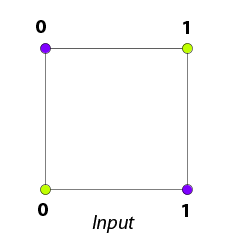
\includegraphics[scale=0.6]{3a_input.png}
        \caption{Complejo de entrada.}
      \end{figure}
      
      \begin{figure}
        \centering
        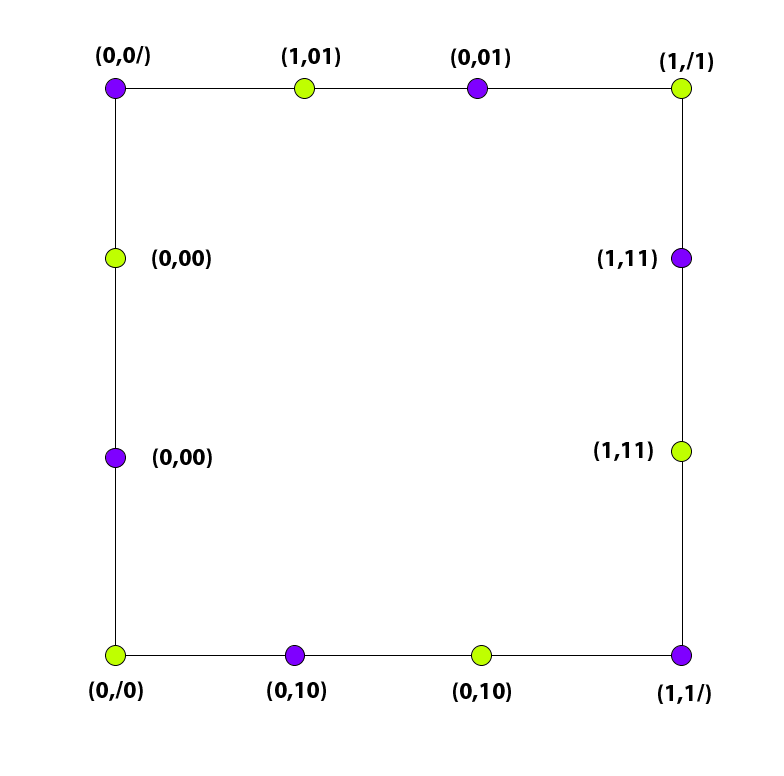
\includegraphics[scale=0.26]{3a_protocol.png}
        \caption{Complejo de la segunda ronda.}
      \end{figure}
          
      En la primera ronda(\textit{figura 2}) podemos decir que el complejo es el mismo
      al del problema visto en clase, esto se debe a que cada proceso ocupa el único espacio
      de memoria del cual dispone, teniendo como información inicial, lo que él dijo (0 ó 1)
      más aparte lo que leyo del otro proceso (0, 1 ó $\perp$).\\
      Lo interesante ocurre apartir de la ronda 2, ¿cuál es el complejo que resulta en la segunda
      ronda?, la respuesta es simple, el mismo complejo de la ronda 1. Aún más interesante
      ¿por que ocurre esto?, primero debemos notar que en el modelo \textit{full information} 
      saber toda la historia de la conversación que mantuvieron los dos procesos durante las M
      rondas nos da la capacidad de convertir una arista en 3 posibles mundos subsecuentes,
      como en el modelo que se nos pide en este ejercicio perdemos esa capacidad, entonces 
      no importa cuantas rondas de comuncación mantuvieron los procesos, si en todo momento solo
      existe la posibilidad de que alguno de los dos no escucho al otro o ambos se escucharon.\\
      Por lo tanto, la gráfica de vistas de la ronda M es el mostrado en la \textit{figura 2}.\\
    }
       
      \item{\textsl{¿Cuál es la mejor $\epsilon$ que puede resolver en la tarea del 
            $\epsilon$-agreement en M rondas?}\\ \\
         
          \begin{figure}
            \centering
            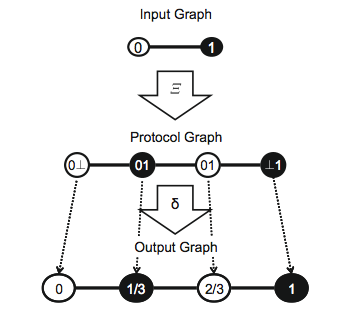
\includegraphics[scale=0.65]{3b_agreement.png}
            \caption{Mapeo simplicial para resolver \textit{3-approximate agreement}}
          \end{figure}
          
          En clase vimos que si $M = 2$, entonces la $\epsilon$ más fina que podemos obtener es
          $1/3$, la razón de esto es por que topologicamente si la grafica de salida tuviera 
          más de 4 vértices, la gráfica de protocolo no se puede mapear a la de salida.\\
          En este ejercicio se nos pide analizar el caso en que Alice dice 0 y Bob dice 1 para M
          rondas. Por el inciso \textit{a} sabemos que la grafica de protocolo para cualquier
          M es igual a la grafica de protocolo de $M = 2$, por lo que la $\epsilon$-agreement 
          óptima para M rondas es la $\epsilon$ para $M = 2$ y usando el mismo razónamiento
          decirmos que la $\epsilon$ óptima es $1/3$.\\
          Por último el mapeo simplicial es el mismo al visto en clase: 
          
          \begin{itemize}
            \item{Si Alice o Bob no escucharon al otro proceso, entonces deciden lo que en un principio
              dijeron.}
            \item{Si Bob sabe que dijo Alice, entonces decide $1/3$.}
            \item{Si Alice sabe que dijo Bob, entonces decide $2/3$.}
          \end{itemize}

          
          
        }
        
      \end{enumerate}
    }
    
  \end{enumerate}
\end{document}